\documentclass[10pt,landscape]{article}
\usepackage[scaled=0.92]{helvet}
\usepackage{calc,multicol,ifthen}
\usepackage[a4paper,margin=5mm,landscape]{geometry}
\usepackage{amsmath,amsthm,amsfonts,amssymb,mathtools,bm}
\usepackage{color,graphicx,overpic,hyperref}
\usepackage{newtxtext}
\usepackage{enumitem}
\usepackage{braket}
\usepackage[table]{xcolor}
\usepackage{vwcol,tikz,nicematrix}
\usetikzlibrary{arrows.meta,calc}
\usepackage[T1]{fontenc}
\usepackage{cancel,mathrsfs,listings}
\setlist{nosep}
\lstset{language=Java,keywordstyle={\bfseries\color{black}}}
\pagestyle{empty}
\newenvironment{tightcenter}{\setlength\topsep{0pt}\setlength\parskip{0pt}\begin{center}}{\end{center}}
\makeatletter
\renewcommand{\section}{\@startsection{section}{2}{0mm}{-1ex plus -.5ex minus -.2ex}{0.5ex plus .2ex}{\normalfont\normalsize\bfseries}}
\renewcommand{\subsection}{\@startsection{subsection}{3}{0mm}{-1ex plus -.5ex minus -.2ex}{1ex plus .2ex}{\normalfont\small\bfseries}}
\renewcommand{\familydefault}{\sfdefault}
\renewcommand\rmdefault{\sfdefault}
\renewcommand{\labelenumii}{\theenumii}
\renewcommand{\theenumii}{\theenumi.\arabic{enumii}.}
\renewcommand\labelitemii{•}
\renewcommand{\lnot}{\mathord{\sim}}
\renewcommand{\bf}[1]{\textbf{#1}}
\newcommand{\abs}[1]{\vert #1 \vert}
\newcommand{\Mod}[1]{\ \mathrm{mod}\ #1}
\makeatother
\definecolor{myblue}{cmyk}{1,.72,0,.38}
\everymath\expandafter{\the\everymath \color{myblue}}
\newcommand{\vct}[1]{\bm{#1}}
\newcommand{\dd}{\,\mathrm d}
\newcommand{\e}{\mathrm e}
\newcommand{\er}{\hat{\vct e}_r}
\newcommand{\et}{\hat{\vct e}_\theta}
\setcounter{secnumdepth}{0}
\setlength{\parindent}{0pt}
\setlength{\parskip}{0pt plus 0.5ex}
\setlength{\leftmargini}{0.5cm}
\setlength{\leftmarginii}{0.5cm}
\setlist[itemize,1]{leftmargin=2mm,labelindent=1mm,labelsep=1mm}
\setlist[itemize,2]{leftmargin=4mm,labelindent=1mm,labelsep=1mm}
\newtheorem{example}[section]{Example}
\begin{document}

\raggedright\footnotesize
\setlength{\columnseprule}{0.25pt}
\setlength{\premulticols}{1pt}
\setlength{\postmulticols}{1pt}
\setlength{\multicolsep}{1pt}
\setlength{\columnsep}{2pt}
\begin{multicols*}{4}

\begin{center}
    \fbox{%
        \parbox{0.8\linewidth}{\centering \textcolor{black}{
            {\Large\textbf{PC2032}}
            \\ \normalsize{AY26/27 Sem 1}}
            \\ {\footnotesize \textcolor{myblue}{by Boon How}} 
        }%
    }
\end{center}

% ====================================================
%                   Start Cheatsheet
% ====================================================

\section{0. Before algebra: choose a model}
\begin{itemize}
    \item \textbf{Draw:} chosen system, axes, all real forces, known and requested quantities. Use one FBD per body when forces differ.
    \item \textbf{Translate event words:} loses contact $\Rightarrow N=0$; impending slip $\Rightarrow |f_s|=\mu_sN$; turning point/highest point/max compression $\Rightarrow v=0$; no slip $\Rightarrow v_{\rm CM}=R\omega$.
    \item \textbf{Choose:} forces/constraints $\Rightarrow\sum\vct F=m\vct a$; speeds/heights/springs $\Rightarrow K_i+U_i+W_{\rm nc}=K_f+U_f$; short impact $\Rightarrow\Delta\vct P=\vct J_{\rm ext}$; mass joining/leaving $\Rightarrow$ fixed-material-set momentum balance.
    \item \textbf{Check:} units, sign, limiting case and physical root. Negative time, distance or speed is normally rejected.
    \item \textbf{Recognise:} You are stuck. \textbf{Write:} Write the target at the top ($N?\ v?\ t?\ \theta?\ I?$). Keep only equations containing it. \textbf{Get:} A one-line physical claim: e.g. contact holds because $N\ge0$.
\end{itemize}

\section{1. Kinematics, projectiles, and circular motion}
\begin{itemize}
    \item \textbf{Definitions and dimensions.} $\vct v=\dd\vct r/\dd t$, $\vct a=\dd\vct v/\dd t$; $[v]=LT^{-1}$, $[a]=LT^{-2}$. \\
    For constant $a$:
    \[
    \begin{gathered}v=v_0+at,\quad x=x_0+v_0t+\tfrac12at^2\\v^2=v_0^2+2a(x-x_0).\end{gathered}
    \]
    \item \textbf{Constant angular acceleration $\alpha$.}
    \[
    \begin{gathered}\omega=\omega_0+\alpha t\\\theta=\theta_0+\omega_0t+\tfrac12\alpha t^2\\\omega^2=\omega_0^2+2\alpha(\theta-\theta_0).\end{gathered}
    \]
    \item \textbf{Projectile.} Resolve at once:
    \[
    x=x_0+v_0\cos\theta\,t,\qquad y=y_0+v_0\sin\theta\,t-\tfrac12gt^2.\]
    \begin{tightcenter}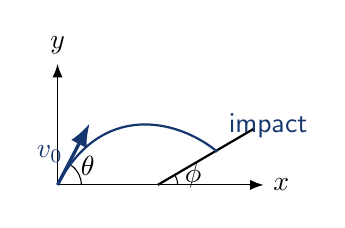
\begin{tikzpicture}[scale=.48,>=Latex]
    \draw[->] (0,0)--(5.45,0) node[right] {$x$}; \draw[->] (0,0)--(0,3.2) node[above] {$y$};
    \draw[thick] (2.65,0)--(5.2,1.49); \draw[myblue,thick] (0,0)..controls (1.15,2.2) and (3.15,1.75)..(4.2,.90);
    \fill[myblue] (4.2,.90) circle (1.25pt) node[above right=1pt] {impact};
    \draw[->,myblue,very thick] (0,0)--(.85,1.63) node[midway,left] {$v_0$};
    \draw (0.63,0) arc[start angle=0,end angle=55,radius=.63] node[right] {$\theta$};
    \draw (3.18,0) arc[start angle=0,end angle=30,radius=.5] node[right] {$\phi$};
    \end{tikzpicture}\end{tightcenter}
    \item\textbf{Recognise:} Projectile meets a slope. \textbf{Write:} At impact use $(x,y)=(d\cos\phi,d\sin\phi)$ in both equations; eliminate $t$ before optimising. \textbf{Get:} For maximum upslope distance: $\theta_*=\tfrac12(\pi/2+\phi)$ and $d_{\max}=v_0^2(1-\sin\phi)/(g\cos^2\phi)$.
    \item \textbf{Recognise:} Cliff launch. \textbf{Write:} Solve $y(t)=y_{\rm ground}$ and keep $t>0$ first. \textbf{Get:} Then $R=(v_0\cos\theta)t$.
    \item \textbf{Polar / circle.}
    \[
    \vct v=\dot r\er+r\dot\theta\et,\quad \vct a=(\ddot r-r\dot\theta^2)\er+(r\ddot\theta+2\dot r\dot\theta)\et.
    \]
    The polar basis rotates: $\dot{\er}=\dot\theta\et$, $\dot{\et}=-\dot\theta\er$. On $r=R$: $a_r=-v^2/R=-R\dot\theta^2$, $a_t=\dot v=R\ddot\theta=v\,\dd v/\dd s$; $T=2\pi/|\omega|=2\pi R/v$. Uniform circular motion has $a_t=0$, \emph{not} $\vct a=0$.
\end{itemize}

\section{2. Relative motion and inertial / rotating frames}
\begin{itemize}
    \item \textbf{Non-rotating frames.}
    \[
    \vct v_{P/A}=\vct v_{P/B}+\vct v_{B/A},\qquad \vct a_{P/A}=\vct a_{P/B}+\vct a_{B/A}.
    \]
    \item \textbf{The full inertial acceleration formula.} If a frame has origin acceleration $\vct a_O$ and angular velocity $\vct\Omega$,
    \[
    \boxed{\begin{gathered}\vct a_{\rm inertial}=\vct a_{\rm rot}+\vct a_O\\+\dot{\vct\Omega}\!\times\!\vct r+2\vct\Omega\!\times\!\vct v_{\rm rot}\\+\vct\Omega\!\times(\vct\Omega\!\times\!\vct r)\end{gathered}}.
    \]
    Terms after $\vct a_O$: Euler, Coriolis, centrifugal. Also $\vct v_{\rm inertial}=\vct v_O+\vct\Omega\times\vct r+\vct v_{\rm rot}$.
    \item \textbf{Recognise:} Question gives a rotating platform/frame. \textbf{Write:} Write $\vct\Omega$, $\vct r$, and $\vct v_{\rm rot}$ at the named instant. Draw each cross product; do not guess its sign. \textbf{Get:} Coriolis has $+2\vct\Omega\times\vct v_{\rm rot}$ in the inertial acceleration transformation, but the rotating-frame fictitious acceleration/force is $\vct a_{\rm Cor}=-2\vct\Omega\times\vct v_{\rm rot}$ and $\vct F_{\rm Cor}=-2m\vct\Omega\times\vct v_{\rm rot}$. It vanishes when $\vct v_{\rm rot}=0$ or $\vct v_{\rm rot}\parallel\vct\Omega$.    \item \textbf{Rotating-frame fictitious-force form.} $\vct F_{\rm fict}=-m\vct a_O-m\dot{\vct\Omega}\times\vct r-2m\vct\Omega\times\vct v_{\rm rot}-m\vct\Omega\times(\vct\Omega\times\vct r)$. Include these alongside real forces when drawing an FBD in the rotating frame.
    \item \textbf{Translating non-inertial frame.} In the frame, add $\vct F_{\rm fict}=-m\vct a_{\rm frame}$, then apply $\sum\vct F_{\rm real}+\vct F_{\rm fict}=m\vct a_{\rm frame\ coordinates}$.
\end{itemize}

\section{3. Newton's laws, contact, friction, and constraints}
\[
\sum\vct F=m\vct a,\qquad N\ge0,\qquad |f_s|\le\mu_sN.
\]
\[
f_k=\mu_kN,\qquad \vct F_s=-kx\,\hat x.
\]
\begin{tightcenter}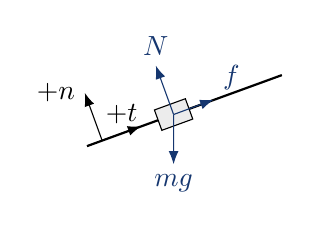
\begin{tikzpicture}[scale=.55,>=Latex]
\draw[thick] (0,0)--(4.5,1.64);
\begin{scope}[rotate around={20:(2,.73)}]\draw[fill=gray!15] (1.62,.48) rectangle (2.38,.98);\end{scope}
\coordinate (C) at (2,.73);
\draw[->,myblue] (C)--(1.59,1.86) node[above] {$N$};
\draw[->,myblue] (C)--(2.92,1.07) node[above right] {$f$};
\draw[->,myblue] (C)--(2,-.42) node[below] {$mg$};
\draw[->] (.35,.13)--(1.25,.46) node[midway,above] {$+t$};
\draw[->] (.35,.13)--(-.05,1.23) node[left] {$+n$};
\end{tikzpicture}\end{tightcenter}

\begin{itemize}    \item \textbf{Spring forces.} Hooke's law: $\vct F_s=-kx\,\hat x$ (restoring force), with $U_s=\tfrac12kx^2$. For $F_s=-(ax+bx^2)$ when $x>0$, use $U(x)=\int_0^x(ax'+bx'^2)\dd x'=\tfrac12ax^2+\tfrac13bx^3$, not $\tfrac12kx^2$.
    \item \textbf{Quadratic drag.} In a stationary fluid, $\vct F_D=-kv\vct v$ (opposite to velocity); for downward terminal motion, $v_t=\sqrt{mg/k}$.
    \item \textbf{Free-Body Diagram (FBD).} Isolate one object and draw every real force on it: weight, normal, friction, tension, spring/applied force and drag. A normal is perpendicular to the surface, not automatically $mg$. Static friction is an unknown that adjusts; use equality only at threshold. On a straight incline, $N=mg\cos\theta$ only when no other normal forces/acceleration are present.
    \item \textbf{Ideal rope/pulley constraint.} For a taut inextensible rope, $L=\sum_i(\text{signed segment lengths})=\text{constant}$, hence $\dot L=0$ and $\ddot L=0$. Write this before solving connected-body accelerations.
    \item \textbf{Vertical circle survival.} For an object inside a frictionless loop, $v_{\rm top}\ge\sqrt{gR}$; by energy, $v_{\rm bottom}\ge\sqrt{5gR}$ for just-maintained contact at the top.

    \item \textbf{Recognise:} Contact on a loop, bowl, or curved track. \textbf{Write:} Energy $\to v$ at the named point, then resolve inward: $\sum F_n=mv^2/R$. \textbf{Get:} At detachment set $N=0$. If contact must remain, solve $N(\theta)$ and require $N\ge0$ throughout.
    \item \textbf{Recognise:} Block on wedge / linked bodies. \textbf{Write:} One FBD and component equations per body. Add the geometric condition: no relative acceleration perpendicular to the surface. \textbf{Get:} You obtain all accelerations and contact forces; do not invent conservation of energy if an external push acts.
    \item \textbf{Recognise:} Motorcycle or object speeding around a circle. \textbf{Write:} Split friction: $f_r=mv^2/R$, $f_t=m\dot v=mv\,\dd v/\dd s$. \textbf{Get:} Require $f_r^2+f_t^2\le(\mu_sN)^2$.
\end{itemize}

\section{4. Work, energy, power, and potentials}
\[
W_{A\to B}=\int_A^B\vct F\cdot\dd\vct r,\qquad \Delta K=W_{\rm net},\qquad P=\vct F\cdot\vct v.
\]
\[
\begin{gathered}K_i+U_i+W_{\rm non-conservative}=K_f+U_f\\\Delta U=-W_{\rm conservative},\qquad \vct F=-\nabla U\end{gathered}
\]
\[
F(x)=-\dd U/\dd x,\qquad U_g=mgy,\qquad U_s=\tfrac12kx^2.
\]
\[U_N=-GMm/r,\qquad \vct F_G=-GMm\,\hat r/r^2.
\]

\begin{itemize}
    \item \textbf{Line integral.} Parameterise the actual path, write $\dd\vct r=\dd x\hat\imath+\dd y\hat\jmath+\dd z\hat k$, then evaluate $\vct F\cdot\dd\vct r$. A conservative field has $\int \vct F\cdot\dd\vct r=0$.
    \begin{tightcenter}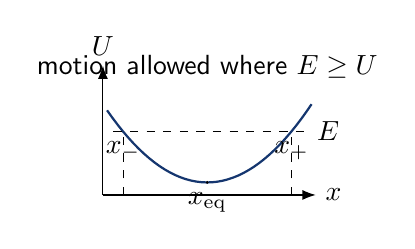
\begin{tikzpicture}[scale=.53,>=Latex]
    \draw[->] (0,0)--(5.1,0) node[right] {$x$}; \draw[->] (0,0)--(0,3.1) node[above] {$U$};
    \draw[myblue,thick,domain=.10:5.0,samples=40] plot (\x,{.30*(\x-2.5)^2+.30});
    \draw[dashed] (.25,1.52)--(4.9,1.52) node[right] {$E$};
    \draw[dashed] (.484,0)--(.484,1.52) node[below] {$x_-$}; \draw[dashed] (4.516,0)--(4.516,1.52) node[below] {$x_+$};
    \fill (2.5,.30) circle (1pt) node[below] {$x_{\rm eq}$}; \node[above] at (2.5,2.55) {motion allowed where $E\ge U$};
    \end{tikzpicture}\end{tightcenter}
    \item \textbf{Read a potential graph.} Turning points: $E=U$ and $v=0$; speed largest at smallest accessible $U$; equilibrium has $U'(x_{\rm eq})=0$; minimum is stable, maximum unstable.    \item \textbf{Small oscillations / SHM.} Near stable $x_{\rm eq}$, let $q=x-x_{\rm eq}$: $U\approx U_{\rm eq}+\tfrac12U''(x_{\rm eq})q^2$, $\ddot q=-\omega^2q$, $\omega=\sqrt{U''(x_{\rm eq})/m}$. Hence $q=A\cos(\omega t+\phi)$, $T=2\pi/\omega$, and $f=1/T=\omega/(2\pi)$.
    \item \textbf{Recognise:} Time through a 1-D potential. \textbf{Write:} Find $E$ from the release condition. \textbf{Get:}  $t=\int_{x_i}^{x_f}\sqrt{m/[2(E-U(x))]}\,\dd x$; near a smooth potential maximum the integral may diverge.
\end{itemize}

\section{5. Momentum, collisions, and variable mass}
\[
\begin{gathered}\vct p=m\vct v,\qquad \vct J=\int\vct F_{\rm ext}\dd t=\Delta\vct P\\\frac{\dd\vct P}{\dd t}=\sum\vct F_{\rm ext}\end{gathered}
\]
\[
\vct P=M\vct V_{\rm CM}.
\]

\begin{itemize}
    \item \textbf{Recognise:} Short collision. \textbf{Write:} Choose the two (or more) bodies as one system. If external impulse is negligible, write momentum components before anything else. \textbf{Get:}  $\sum\vct p_i=\sum\vct p_f$; in 2-D write separate $x$ and $y$ equations. Add $K_i=K_f$ \emph{only} if elastic.
    \item \textbf{One-dimensional elastic collision.}
    \[
    v_{1f}=\frac{(m_1-m_2)v_{1i}+2m_2v_{2i}}{m_1+m_2}.
    \]
    \[
    v_{2f}=\frac{2m_1v_{1i}+(m_2-m_1)v_{2i}}{m_1+m_2}.
    \]    \item \textbf{Collision shortcuts.} In a 1-D elastic collision, $v_{1i}-v_{2i}=-(v_{1f}-v_{2f})$ (relative speed reverses). Perfectly inelastic: $V=(m_1v_{1i}+m_2v_{2i})/(m_1+m_2)$ and $K_i-K_f=\tfrac12\mu|\vct v_{1i}-\vct v_{2i}|^2$, where $\mu=m_1m_2/(m_1+m_2)$.
    \item \textbf{Centre-of-mass frame.} $\vct V_{\rm CM}=\sum_i m_i\vct v_i/\sum_i m_i$. Transform velocities by $\vct u_i=\vct v_i-\vct V_{\rm CM}$. In this frame total momentum is zero; for an elastic collision, each $|\vct u_i|$ is unchanged and only direction changes.
    \item \textbf{Recognise:} Maximum two-dimensional scattering angle. \textbf{Write:} Move to the CM frame; rotate the fixed-length outgoing $\vct u$ vector, then add $\vct V_{\rm CM}$ back. \textbf{Get:} The extreme lab direction is the tangent from the origin to the allowed velocity circle.
    \item \textbf{Mass crossing a boundary.} Do not use fixed-mass $F=m\vct a$ blindly. Over $\dd t$, select a \emph{fixed material set} containing the mass about to enter/leave, then apply impulse. For rain initially at rest:
    \[
    \begin{gathered}(m+\dd m)(v+\dd v)-mv=mg\dd t\\\text{(retain first-order terms)}\end{gathered}
    \]    \item \textbf{Variable mass / rocket.} If $\vct u_{\rm rel}$ is the velocity of exchanged mass relative to the object, $m\,\dd\vct v/\dd t=\vct F_{\rm ext}+\vct u_{\rm rel}\,\dd m/\dd t$. For a rocket with no external force and exhaust speed $u$, $\Delta v=u\ln(m_i/m_f)$.
\end{itemize}

\section{6. Centre of mass: the integration method}
\[
\boxed{\begin{gathered}\vct r_{\rm CM}=\frac{\sum_i m_i\vct r_i}{M}=\frac1M\int\vct r\,\dd m\\\sum\vct F_{\rm ext}=M\vct a_{\rm CM}\end{gathered}}.
\]

\begin{itemize}
    \item \textbf{Choose $\dd m$ to match the object:} thin rod $\dd m=\lambda(x)\dd x$; lamina $\dd m=\sigma(x,y)\dd A$; volume $\dd m=\rho(x,y,z)\dd V$. Cylindrical: $\dd V=r\dd r\dd\phi\dd z$; spherical: $\dd V=r^2\sin\theta\dd r\dd\theta\dd\phi$.
    \item\textbf{Recognise:} Any CM integral. \textbf{Write:} (1) Use symmetry first. (2) Write $M=\int\dd m$. (3) Write the relevant numerator $x_{CM} = \int x\dd m$, $y_{CM} = \int y\dd m$, or $y_{CM} = \int z\dd m$. \textbf{Get:} Divide numerator by $M$. Never cancel a non-uniform density such as $kxy$ before integrating.
    \begin{tightcenter}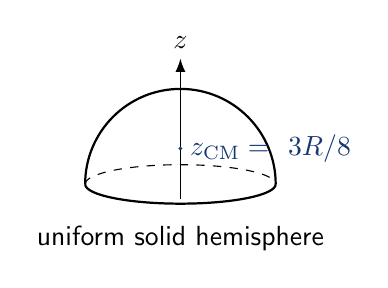
\begin{tikzpicture}[scale=.55,>=Latex]
    \draw[thick] (0,0) arc[start angle=180,end angle=0,x radius=2.2,y radius=2.2];
    \draw[dashed] (0,0) arc[start angle=180,end angle=0,x radius=2.2,y radius=.45];
    \draw[thick] (0,0) arc[start angle=180,end angle=360,x radius=2.2,y radius=.45];
    \draw[->] (2.2,-.35)--(2.2,2.9) node[above] {$z$}; \fill[myblue] (2.2,.825) circle (1.3pt) node[right] {$z_{\rm CM}= \hspace{4pt} 3R/8$};
    \node[below] at (2.2,-.75) {uniform solid hemisphere};
    \end{tikzpicture}\end{tightcenter}
    \item \textbf{Support/tipping.} A body can remain statically supported only while the vertical line through its CM lies inside the support region. For a hemisphere, symmetry gives $x_{\rm CM}=y_{\rm CM}=0$; integrating $z\rho\dd V$ gives $z_{\rm CM}=3R/8$ above its flat face.
\end{itemize}

\section{7. Rigid bodies, torque, inertia, and rolling}
\[\vct v_P=\vct v_O+\vct\omega\times\vct r_{P/O},
\]
\[
\vct a_P=\vct a_O+\vct\alpha\times\vct r_{P/O}+\vct\omega\times(\vct\omega\times\vct r_{P/O}),
\]
\[
\vct\tau_O=\vct r\times\vct F.
\]

\[
\begin{gathered}\sum\tau_O=I_O\alpha\quad\text{(fixed axis)}\\I=\int s^2\dd m,\qquad I=I_{\rm CM}+Md^2\end{gathered}
\]
\[
K_{\rm rot}=\tfrac12I\omega^2,\qquad K=\tfrac12Mv_{\rm CM}^2+\tfrac12I_{\rm CM}\omega^2.
\]

\begin{itemize}
    \item For planar lamina (2D) axes through one point: $I_z=I_x+I_y$. State the axis; $s$ is its \emph{perpendicular} distance. Standard $I$: rod centre $ML^2/12$; rod end $ML^2/3$; hoop $MR^2$; disk/cylinder $MR^2/2$; sphere $2MR^2/5$; spherical shell $2MR^2/3$.
    \item \textbf{Worked inertia pattern: square wire about its centre.} Split the square into four rods: each has $m=M/4$, length $L$, and its own centre is distance $d=L/2$ from the square centre.
    \begin{tightcenter}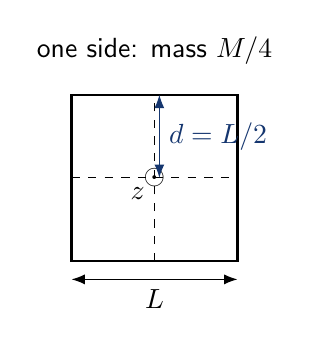
\begin{tikzpicture}[scale=.62,>=Latex]
    \draw[thick] (0,0) rectangle (3.4,3.4);
    \draw[dashed] (1.7,0)--(1.7,3.4) (0,1.7)--(3.4,1.7);
    \node at (1.7,1.7) {$\odot$};
    \node[below left] at (1.7,1.7) {$z$};
    \draw[<->] (0,-.38)--(3.4,-.38) node[midway,below] {$L$};
    \draw[<->,myblue] (1.8,1.7)--(1.8,3.4) node[midway,right] {$d=L/2$};
    \node[above] at (1.7,3.82) {one side: mass $M/4$};
\end{tikzpicture}\end{tightcenter}
    The rod formula is about its \emph{own} centre, so shift it to the required square-centre axis: $I_{\rm side}=I_{\rm rod,CM}+md^2=\frac{(M/4)L^2}{12}+\frac M4(\frac L2)^2=\frac{ML^2}{12}$. Add the four side contributions: $I_z=4I_{\rm side}={ML^2/3}$. \emph{Chain: split object $\to$ find each piece mass $\to$ use its known $I_{\rm CM}$ $\to$ add $md^2$ $\to$ sum.}
    \begin{tightcenter}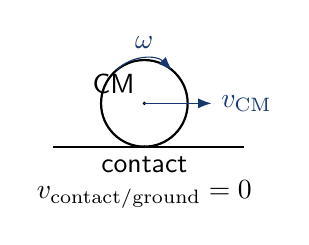
\begin{tikzpicture}[scale=.55,>=Latex]
    \draw[thick] (0,0)--(4.4,0); \draw[thick] (2.1,1) circle (1); \fill (2.1,1) circle (1.2pt) node[above left] {CM}; \fill (2.1,0) circle (1pt) node[below] {contact};
    \draw[->,myblue] (2.1,1)--(3.65,1) node[right] {$v_{\rm CM}$};
    \draw[->,myblue] (1.46,1.77) arc[start angle=135,end angle=45,radius=.9] node[midway,above] {$\omega$};
    \node[below] at (2.1,-.55) {$v_{\rm contact/ground}=0$};
    \end{tikzpicture}\end{tightcenter}    \item \textbf{Rolling without slip.} The contact condition is $\vct v_{\rm CM}+\vct\omega\times\vct r_{\rm contact/CM}=0$. For rightward rolling, $\vct\omega=-\omega\hat k$ (clockwise), so $v_{\rm CM}=R\omega$ and (constant $R$) $a_{\rm CM}=R\alpha$. The contact point has zero \emph{velocity}, not necessarily zero acceleration. For rolling down an incline of angle $\beta$, $a_{\rm CM}=g\sin\beta/[1+I_{\rm CM}/(MR^2)]$. First calculate the \emph{required} static friction, then check $|f_s|\le\mu_sN$; otherwise it slips and the relation fails.    \item \textbf{Angular momentum and rotational work.} $\vct L_O=\sum\vct r_i\times\vct p_i$, $\dd\vct L_O/\dd t=\sum\vct\tau_O$; hence $\sum\vct\tau_{\rm ext,O}=0\Rightarrow\vct L_O=\text{constant}$. For fixed-axis motion $L=I\omega$. Also $W_{\rm rot}=\int\tau\dd\theta$ and $P_{\rm rot}=\tau\omega$.
    \item \textbf{Velocity of any point on a rolling wheel.} Use $\vct v_P=\vct v_{\rm CM}+\vct\omega\times\vct r_{P/\rm CM}$, not a memorised speed. For rightward rolling, the top point has $2v_{\rm CM}$ and the contact point $0$.
    \item \textbf{Recognise:} Tilted rod axis. \textbf{Write:} Draw the axis and express perpendicular distance as $s=|x|\sin\theta$. \textbf{Get:} Uniform rod through centre: $I=\tfrac1{12}ML^2\sin^2\theta$.
    \item \textbf{Recognise:} Rope lifted at constant speed. \textbf{Write:} Moving mass $m=\lambda y$. Include support of hanging piece and momentum rate of fresh rope. \textbf{Get:}  $F=\lambda yg+\lambda v_0^2$ under the tutorial model.
\end{itemize}

\section{8. Extra lecture models and quick checks}
\begin{itemize}
    \item \textbf{Dimensional analysis.} Assume $v\propto B^a\rho^b$, substitute $[B]=ML^{-1}T^{-2}$ and $[\rho]=ML^{-3}$, then equate exponents. Example: $v\propto\sqrt{B/\rho}$.
    \item \textbf{Linear drag.} With downward positive and $\vct F_{\rm drag}=-k\vct v$ in a fluid at rest, $\tau=m/k$:
    \[
    \begin{gathered}v(t)=g\tau+(v_0-g\tau)\e^{-t/\tau}\\v_{\rm terminal}=g\tau=mg/k\end{gathered}
    \]
    \item \textbf{Recognise:} Linear ODE / trial solution. \textbf{Write:} Try $x=A\e^{\lambda t}$. \textbf{Get:} Substitute to get the characteristic polynomial; each root supplies a solution and superposition gives the general result.
    \item \textbf{Spring and rough ground.} When compression is $x$, friction may act over the whole travelled distance, e.g. $L+x$, not merely $L$. At rest after compression, test $kx\le\mu_smg$ before deciding whether it moves back.
    \item \textbf{Curved ramp.} If slope angle varies with arc length, $\dd y=\sin\theta(s)\dd s$, so $W_g=-mg\int\sin\theta(s)\dd s$ and (when given $N=mg\cos\theta$) $W_f=-\int\mu_kN\dd s$.
    \item \textbf{Coupled spring oscillation.} If a small displacement makes masses $m$ and $M$ move together, use the total effective inertia: $\omega=\sqrt{k/(m+M)}$; gravity shifts equilibrium but not this $\omega$.
\end{itemize}

\section{9. Universal answer skeleton}
\begin{enumerate}[leftmargin=3.5mm,itemsep=.3pt,topsep=1pt]
\item State \textbf{system, axes, and positive direction}. Draw the diagram before equations.
\item State the \textbf{event/constraint}: contact? slip? impact? turning point? no-slip? fixed length?
\item Write the \textbf{governing principle} first: $\sum F=ma$, energy, impulse-momentum, CM, or rotation.
\item Substitute only after the equations are visible. Solve, then use units and a physical condition ($N\ge0$, $E\ge U$, $t>0$, etc.) to choose the valid root.
\end{enumerate}

\section{10. Assignment patterns: the missing first steps}
\begin{itemize}
    \item \textbf{Tangential versus normal acceleration.} If $\vct r(t)$ is given, differentiate twice. The part that changes speed is not generally $|\vct a|$:
    \[
    \begin{gathered}a_t=\frac{\vct a\cdot\vct v}{|\vct v|}=\frac{\dd|\vct v|}{\dd t}\\a_n=\frac{|\vct v\times\vct a|}{|\vct v|}=\frac{v^2}{R}\end{gathered}
    \]
    \item \textbf{Use:} in a vertical circle, use energy for speed, then a separate radial equation. Choose the radial positive direction first; at loss of contact $N=0$, \emph{not} $v=0$. For an inside track at the top (inward downward),
    \[
    \begin{gathered}mg+N=\frac{mv_t^2}{R},\\v_b^2=v_t^2+4gR.\end{gathered}
    \]
    \item \textbf{Rigid link / moving wedge.} A fixed separation gives a constraint before conservation laws:
    \[
    \begin{gathered}(\vct v_i-\vct v_j)\cdot(\vct r_i-\vct r_j)=0,\\(\vct a_i-\vct a_j)\cdot(\vct r_i-\vct r_j)=-|\vct v_i-\vct v_j|^2.\end{gathered}
    \]
    For a block that stays on a moving wedge, the relative acceleration has no normal component: $\vct a_{\rm block/wedge}\cdot\hat n=0$. Draw one FBD per body, then apply this condition.
    \item \textbf{Non-uniform centre of mass.} Put the density inside $\dd m$; it does \emph{not} cancel. For a rod,
    \[
    x_{\rm CM}=\frac{\int x\lambda(x)\dd x}{\int\lambda(x)\dd x};\]
    for a lamina use $\dd m=\sigma(x,y)\dd A$. Symmetry can remove a whole coordinate before integrating.
    \item \textbf{Collision followed by spring compression.} At \emph{maximum} compression, colliding bodies share a velocity; it is usually not zero:
    \[
    V=\frac{m_1v_{1i}+m_2v_{2i}}{m_1+m_2},\qquad v_1=v_2=V.
    \]
    Use momentum to obtain $V$, then use energy from that instant to include $\tfrac12kx^2$.
    \item \textbf{Small oscillations beyond Hooke's law.} First find equilibrium $F(x_{\rm eq})=0$. With $q=x-x_{\rm eq}$ and a stable equilibrium $F'(x_{\rm eq})<0$,
    \[
    \begin{gathered}F\approx F'(x_{\rm eq})q\\\omega^2=-F'(x_{\rm eq})/m=U''(x_{\rm eq})/m\end{gathered}
    \]
    For an angled spring with $L=\sqrt{x^2+D^2}$, project the force along the motion before linearising: $F_x=-k(L-l_0)x/L$.
    \item \textbf{Newtonian gravity and orbit check.} Keep the direction: $\vct F_g=-GMm\hat r/r^2$ and $U=-GMm/r$. For a circular orbit, gravity supplies the radial acceleration, $GMm/r^2=mv^2/r$, hence $v=\sqrt{GM/r}$.
\end{itemize}

\section{11. More tutorial and homework patterns}
\begin{itemize}
    \item \textbf{Multi-stage motion.} Make one row per phase (accelerate, cruise, brake). In a constant-acceleration phase,
    \[
    \Delta x=\tfrac12(v_i+v_f)\Delta t,\qquad v_f=v_i+a\Delta t.
    \]
    Add distances and times only after solving each row. A minimum-time profile reaches its peak speed and immediately brakes: the cruise time is zero.
    \item \textbf{Work on a curved path.} Parameterise the path before integrating: $\dd\vct r=\dd x\hat\imath+\dd y\hat\jmath+\dd z\hat k$. Only the parallel force component contributes. On a curved ramp with arc coordinate $s$,
    \[
    \dd y=\sin\theta(s)\dd s,\qquad W_g=-mg\int\sin\theta(s)\dd s.
    \]
    If kinetic friction acts, include it over the \emph{full} path travelled, including spring compression.
    \item \textbf{Relative gravity / translating frame.} For two nearby bodies, use relative acceleration $\vct a_{M/P}=\vct a_M-\vct a_P$. A common gravitational acceleration cancels in a co-moving translating frame; only their mutual force remains. In a frame with origin acceleration $\vct a_O$, add $\vct F_{\rm fict}=-m\vct a_O$.
    \item \textbf{Immediate-after-release spring question.} A spring's extension cannot change instantaneously. First use the old equilibrium extension to find the spring force at $t=0^+$; only then apply $\sum F=ma$ to each mass.
    \item \textbf{Point velocities on a rolling wheel.} Do not memorise directions; use $\vct v_P=\vct v_{\rm CM}+\vct\omega\times\vct r_{P/{\rm CM}}$. For rightward no-slip rolling, the top point has speed $2v_{\rm CM}$ and the contact point has speed $0$; the frontmost point has components $(v_{\rm CM},-v_{\rm CM})$.
    \item \textbf{Planar lamina inertia.} Pick thin strips and square their \emph{perpendicular} distance to the stated axis: $I=\int s^2\sigma\dd A$. For the isosceles triangular lamina in the tutorial geometry (long-side axis), horizontal strips give $I=ML^2/6$. Always label the axis before quoting any $I$.
    \item \textbf{Cart / person relative speed.} Translate the stated relative velocity to lab velocities before conserving momentum. If a person jumps backward relative to a cart, write $v_r=V-v$ using your chosen positive direction; conservation applies to the cart-person system during the jump.
\end{itemize}

\end{multicols*}
\end{document}